\documentclass[border=12pt,12pt]{standalone}
\usepackage[T1]{fontenc}
\usepackage{lmodern}
\usepackage{xcolor}
\usepackage{tikz}
\usetikzlibrary{shapes.geometric,shapes.multipart,arrows.meta,positioning,fit,calc}
\setlength{\textwidth}{16cm}
\setlength{\linewidth}{16cm}
\tikzset{
  umlclass/.style={rectangle split, rectangle split parts=3, draw, fill=white,
    font=\scriptsize, text width=5.2cm, align=left, inner sep=3pt},
  usecase/.style={ellipse, draw, fill=white, font=\footnotesize, minimum width=3.4cm,
    minimum height=0.8cm, align=center},
  act/.style={rectangle, rounded corners=6pt, draw, fill=white, font=\footnotesize,
    minimum width=4.2cm, minimum height=0.7cm, align=center},
  dec/.style={diamond, draw, fill=white, aspect=2.2, font=\scriptsize, inner sep=1pt, align=center},
  flow/.style={-{Stealth[length=2.2mm]}, thick},
  assoc/.style={-, thick},
  compo/.style={{Diamond[fill=black,length=3mm,width=2mm]}-, thick},
  aggr/.style={{Diamond[open,length=3mm,width=2mm]}-, thick},
  depend/.style={-{Stealth[length=2mm]}, dashed, thick},
  msg/.style={-{Stealth[length=2mm]}, thick},
  ret/.style={-{Stealth[length=2mm]}, dashed},
}
\newcommand{\actor}[2]{% #1 node name, #2 label
  \begin{scope}[shift={(#1)}]
    \draw[thick] (0,0.55) circle (0.18);
    \draw[thick] (0,0.37) -- (0,-0.1);
    \draw[thick] (-0.3,0.2) -- (0.3,0.2);
    \draw[thick] (0,-0.1) -- (-0.22,-0.5);
    \draw[thick] (0,-0.1) -- (0.22,-0.5);
    \node[font=\footnotesize, below] at (0,-0.5) {#2};
  \end{scope}}


\begin{document}
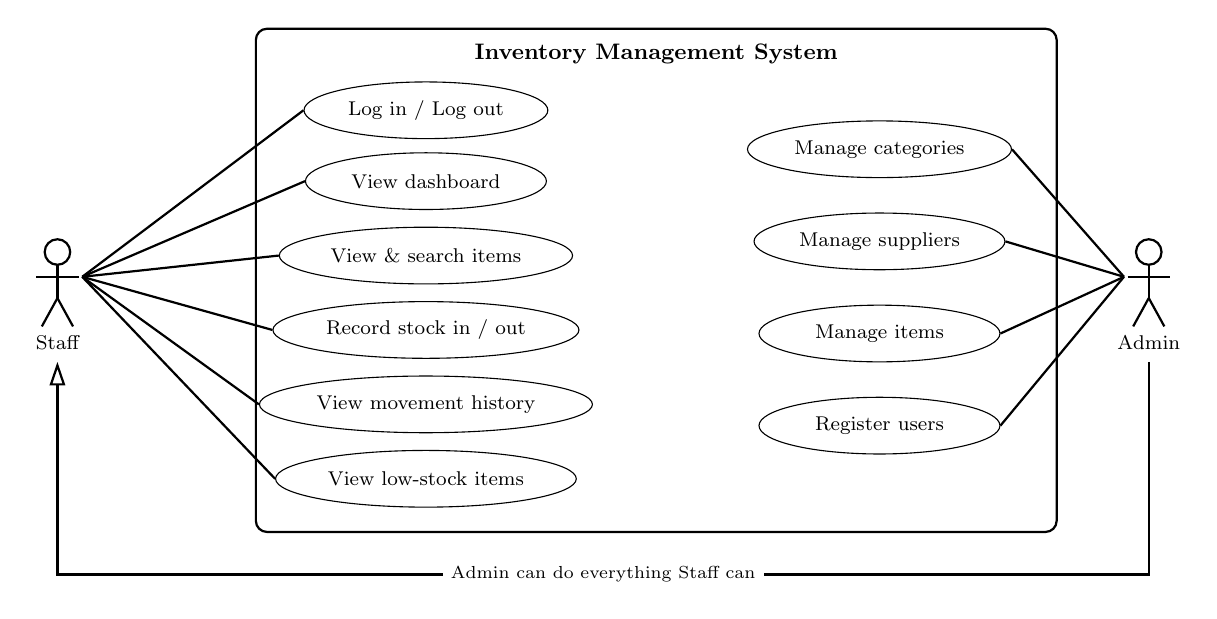
\begin{tikzpicture}[scale=0.9, every node/.style={transform shape}]
  \draw[thick, rounded corners] (-2.4,-6.0) rectangle (8.9,1.1);
  \node[font=\small\bfseries] at (3.25,0.75) {Inventory Management System};
  \node[usecase] (uc1) at (0,-0.05)    {Log in / Log out};
  \node[usecase] (uc2) at (0,-1.05) {View dashboard};
  \node[usecase] (uc3) at (0,-2.1)  {View \& search items};
  \node[usecase] (uc4) at (0,-3.15) {Record stock in / out};
  \node[usecase] (uc5) at (0,-4.2)  {View movement history};
  \node[usecase] (uc6) at (0,-5.25) {View low-stock items};
  \node[usecase] (uc7) at (6.4,-0.6) {Manage categories};
  \node[usecase] (uc8) at (6.4,-1.9) {Manage suppliers};
  \node[usecase] (uc9) at (6.4,-3.2) {Manage items};
  \node[usecase] (uc10) at (6.4,-4.5) {Register users};
  \coordinate (staff) at (-5.2,-2.6);
  \coordinate (admin) at (10.2,-2.6);
  \actor{staff}{Staff}
  \actor{admin}{Admin}
  \foreach \u in {uc1,uc2,uc3,uc4,uc5,uc6} \draw[assoc] (-4.85,-2.4) -- (\u.west);
  \foreach \u in {uc7,uc8,uc9,uc10} \draw[assoc] (9.85,-2.4) -- (\u.east);
  % generalisation: Admin is a Staff (inherits all staff use cases)
  \draw[-{Triangle[open,length=3mm]}, thick] (10.2,-3.6) -- (10.2,-6.6) -- (-5.2,-6.6) -- (-5.2,-3.6);
  \node[font=\scriptsize, fill=white] at (2.5,-6.6) {Admin can do everything Staff can};
\end{tikzpicture}
\end{document}
